\DiaryEntry{Normal Subgroups}{2016-05-10}{Algebra}

A subgroup H of a group G is normal in G if \(gH = Hg\) for all
\(g \in G\). That is, a normal subgroup of a group G is one in which the
right and left cosets are precisely the same.

Let G be a group and N be a subgroup of G. Then the following statements
are equivalent:

\begin{itemize}

\item
  The subgroup N is normal in G.
\item
  For all \(g \in G\) , \(gNg^{-1}\) is a subset of N.
\item
  For all \(g \in G\) , \(gNg^{-1}\) actually is N.
\end{itemize}

If the group G is abelian, then every subgroup of G is a normal
subgroup. This is easy and a strong condition on the group G. More
interesting are non-abelian groups which nevertheless have normal
subgroups. Existence will depend on the group G itself, but also on the
subgroup (i.e.~not all subgroups H of a non-abelian group G are normal).

\subsection{Example}\label{example}

Consider the group \(\mathbb{Z}_6\) with group operation modulo-6
addition and a subgroup \(N=\{0,3\}\).

We need to check that the third condition from above holds.

\begin{itemize}
\item
  For \(g=0\), we have \(g^{-1}=0\) and (i)
  \(g 0 g^{-1}=0 \star 0 \star 0=0\) and (ii)
  \(g 3 g^{-1}=0 \star 3 \star 0 = 3\).
\item
  For \(g=1\), we have \(g^{-1}=5\) and (i)
  \(g 0 g^{-1}=1 \star 0 \star 5=0\) and (ii)
  \(g 3 g^{-1}=1 \star 3 \star 5 = 3\).
\item
  For \(g=2\), we have \(g^{-1}=4\) and (i)
  \(g 0 g^{-1}=2 \star 0 \star 4=0\) and (ii)
  \(g 3 g^{-1}=2 \star 3 \star 4 = 3\).
\item
  For \(g=3\), we have \(g^{-1}=3\) and (i)
  \(g 0 g^{-1}=3 \star 0 \star 3=0\) and (ii)
  \(g 3 g^{-1}=3 \star 3 \star 3 = 3\).
\item
  For \(g=4\), we have \(g^{-1}=2\) and everything is the same as for
  \(g=2\).
\item
  For \(g=5\), we have \(g^{-1}=1\) and everything is the same as for
  \(g=1\).
\end{itemize}

\subsection{Coset Multiplication}\label{coset-multiplication}

If H is a subgroup of G, then we can define coset multiplication as
\(Ha Hb = H(ab)\). This definition looks very simple, but it is not
clear, whether the product of two cosets defined in this way, is
uniquely defined. E.g. Ha may be the same coset a Hc (this happens when
\(c \in Ha\) and in a similar spirit, Hd may be the same coset as Hb.
Therefore, the product Ha Hb is the same as Hc Hd; however, the coset
H(ab) may not be the same coset as H(cd).

\subsection{Normal Subgroups, Coset Multiplication, and Quotient/Factor
Groups}\label{normal-subgroups-coset-multiplication-and-quotientfactor-groups}

If N is a normal subgroup of G, and if Ha=Hc and Hb=Hd, then
H(ab)=H(cd).

If Ha=Hc, then \(a \in Hc\) and \(a=h_1c\), and similar \(b=h_2d\). The
product \(ab\) then becomes \(ab = h_1 c h_2 d = h_1 (c h_2) d\). But
the left cosets equal the right ones and so we have \(c h_2 = h_3 c\)
and we can rewrite \(ab = h_1 h_3 c d = (h_1 h_3)(c d)\) and this
element is in H(cd). Since \(ab \in H(cd)\), we can deduce that
\(H(ab) = H(cd)\).

The set G/H is the set of all cosets of the subgroup H; i.e.
\(G/H=\{Ha, Hb, Hc, \ldots\}\) and this set forms a group under coset
multiplication:

\begin{itemize}
\item
  The identity element is \(H=He\), as \(Ha He = H(ae) = Ha\).
\item
  The inverse of \(Ha\) is H(a\^{}\{-1\})\$ because
  \(Ha Ha^{-1} = H(a a^{-1}) = He\).
\end{itemize}

Finally, \(G/H\) is a homomorphic image of G. We can choose
\(\phi(x) = Hx\) and this is a homomorphism because
\(\phi(xy) = H(xy) = Hx Hy = \phi(x) \phi(y)\).

\subsubsection{Example}\label{example-1}

Consider \href{\%7Bfilename\%7D2016-03-25-groups_05.markdown}{again} the
group \(\mathbb{Z}_6\) with group operation modulo-6 addition and a
subgroup \(N=\{0,3\}\). The cosets are


\begin{align*}
0 + H = 3 + H &= \{0,3\} \\
1 + H = 4 + H = &= \{1,4\} \\
2 + H = 5 + H &= \{2,5\} \\
\end{align*}


The theorem says that the three items \(0 + H\), \(1 + H\), and
\(2 + H\) form a group. The group operation is
\((a + H) \star (b + H) = (a \star b) + H\).

As an example, \((1+H) \star (0+H) = (1+H)\). The coset \(1+H\) contains
the elements \(\{1,4\}\), the coset \(0+H\) the elements \(\{0,3\}\). If
we combine the element from each coset by means of the group operation,
we obtain \(1+0=1, 1+3=4, 4+0=4, 4+3=1\) and this equals the coset
\(1+H\) as stated.

In a similar spirit, we have \((1+H)\star(2+H)=3+H=0+H\). Combining
elements from \(\{1,4\}\) and \(\{2,5\}\), we obtain
\(1+2=3, 1+5=0, 4+2=0, 4+5=3\) which equals the coset \(0+H\).

Continuing in this spirit, we obtain the operation table as follows:

\[
\begin{array}{c|ccc}
\star & 0+H & 1+H & 2+H \\ \hline
0+H   & 0+H & 1+H & 2+H \\
1+H   & 1+H & 2+H & 0+H \\
2+H   & 2+H & 0+H & 1+H
\end{array}
\]

\subsubsection{Interpretation}\label{interpretation}

In a way, a factor group is a reduction of group elements. Instead of
working with the group elements of N, we consider the cosets of N
instead. The cosets have a ``representative'' and a subgroup. The
``representative'' is the amount the subgroup is shifted by; e.g.~the
coset \(1 + H\) has 1 as ``representative'' and \(H\) is the subgroup -
in other words, the subgroup \(H\) is shifted by 1.

A factor group contains only the ``representative''. If the subgroup
(the cosets are based on) is normal, then the representatives themselves
form a group. The Figure below shows an example of a normal subgroup:
All a-arrows leaving H arrive at the left coset aH; and all arrows
arriving at aH come from the subgroup H. It is this property which
allows to drop the actual elements of the subgroup and consider the
coset ``representative'' instead.

\begin{figure}[H]
\centering
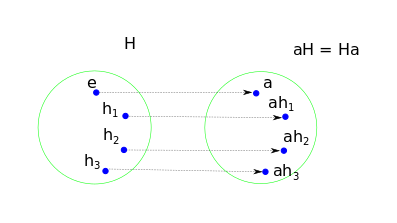
\includegraphics[scale=0.7]{images/groups_10_1.png}
\caption{Page1}
\end{figure}
